% HW Template for CS 6150, taken from https://www.cs.cmu.edu/~ckingsf/class/02-714/hw-template.tex
%
% You don't need to use LaTeX or this template, but you must turn your homework in as
% a typeset PDF somehow.
%
% How to use:
%    1. Update your information in section "A" below
%    2. Write your answers in section "B" below. Precede answers for all 
%       parts of a question with the command "\question{n}{desc}" where n is
%       the question number and "desc" is a short, one-line description of 
%       the problem. There is no need to restate the problem.
%    3. If a question has multiple parts, precede the answer to part x with the
%       command "\part{x}".
%    4. If a problem asks you to design an algorithm, use the commands
%       \algorithm, \correctness, \runtime to precede your discussion of the 
%       description of the algorithm, its correctness, and its running time, respectively.
%    5. You can include graphics by using the command \includegraphics{FILENAME}
%
\documentclass[11pt]{article}
\usepackage{amsmath,amssymb,amsthm}
\usepackage{graphicx}
\usepackage[margin=1in]{geometry}
\usepackage{fancyhdr}
\usepackage{framed}
\usepackage{algorithm}
\usepackage{algpseudocode}
\usepackage{pifont}
\setlength{\parindent}{0pt}
\setlength{\parskip}{5pt plus 1pt}
\setlength{\headheight}{13.6pt}
\newcommand\question[2]{\vspace{.25in}\hrule\textbf{#1}\vspace{.5em}\hrule\vspace{.10in}}
\renewcommand\part[1]{\vspace{.10in}\textbf{(#1)}}
\newcommand\algorith{\vspace{.10in}\textbf{Algorithm: }}
\newcommand\correctness{\vspace{.10in}\textbf{Correctness: }}
\newcommand\runtime{\vspace{.10in}\textbf{Running time: }}
\pagestyle{fancyplain}
\lhead{\textbf{\NAME\ (\UID)}}
\chead{\textbf{HW\HWNUM}}
\rhead{CS 6490, \today}
\begin{document}\raggedright
%Section A==============Change the values below to match your information==================
\newcommand\NAME{Jake Pitkin}  % your name
\newcommand\UID{u0891770}     % your utah UID
\newcommand\HWNUM{5}              % the homework number
%Section B==============Put your answers to the questions below here=======================

\question{Question 1}

\part{a} \textbf{Is it possible to encapsulate an AH packet within an ESP packet and vice versa? Explain with the help of examples.}

Consider the scenario (similar to Figure 17-3 in the text) where Alice and Bob are using IPsec and two firewalls, F1 and F2, between them are also using IPsec. Tunnel mode is used between F1 and F2.

First, the scenario where the firewalls are using AH packets and Alice/Bob are using ESP packets.

\begin{figure}[H]
  \centerline{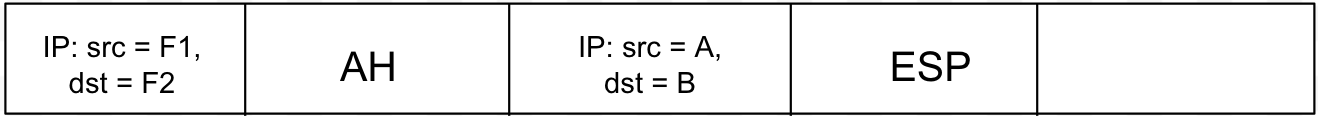
\includegraphics[width=0.5\linewidth]{hw5_1b_1.png}}
\end{figure}

This scenario does \textbf{not} work. One difference of the integrity protection provided by AH/ESP is that AH provides integrity protection of the IP header. The IPsec between F1 and F2 cannot perform the integrity protection of Alice and Bob's IP header as it is inside an encrypted ESP packet and the F1/F2 do not have the key.

Alternatively, the firewalls could be using ESP packets and Alice/Bob are using AH packets.

\begin{figure}[H]
  \centerline{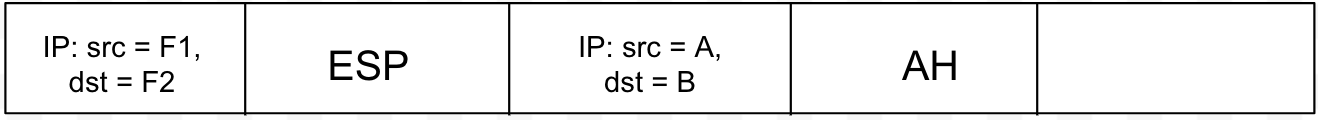
\includegraphics[width=0.5\linewidth]{hw5_1b_2.png}}
\end{figure}

In this scenario, the encapsulation of an AH packet inside a ESP packet \textbf{will} work. The IPsec between the routers are using ESP and do not check the IP headers during the integrity process.


\part{b} \textbf{Suppose Alice is sending packets to Bob using IPsec. Suppose Bob's TCP acknowledgement gets lost, and Alice's TCP, assuming the packet was lost, retransmits the packet. Will Bob's IPsec implementation notice that the packet is a duplicate and discard it?}

Bob's IPsec implementation will \textbf{not} notice it as a duplicate packet. Both AH and ESP IPsec headers have a \textit{sequence number} field that function identically. This sequence number is used by IPsec to prevent replay attacks.

TCP handles the retransmission of packets. When TCP retransmits a packet, AH/ESP will treat it as a new packet with a new sequence number. This is one of the pros of building IPsec on top of TCP: it can hand-off the responsibility of guaranteed delivery (and discarding duplicate packets).

\part{c} \textbf{Referring to Figure 17-2, assume that A and B are using IPsec in transport mode, and F1 and F2 have established an encrypted tunnel using IPsec. Assume A sends a TCP packet to B. Show the relevant fields of the IP header(s) as given to A's IPsec layer, as transmitted by A, as transmitted by F1, and as received by B.}

\part{d} \textbf{Why is IPsec not firewall-friendly?}

A firewall looks at the fields in the transport layer (such as port and protocol) as part of its filtering process. Using the ESP protocol with IPsec encrypts this information and the firewall does not have the ability to decrypt this information. Solutions include terminating IPsec at the firewall or trusting the endpoint and forwarding the encrypted packet to the endpoint.

\question{Question 2}

\part{a} \textbf{Why does the HMAC computation in SSL data transfer phase use a sequence number with each record even though SSL is built on top of TCP that delivers data in the correct order?}

\part{b} \textbf{This question pertains to 3G-UMTS security. Consider the case when a user visits another country and turns her phone on to make a phone call and notices service X. However, it is possble that service provider X is actually service provider Y that charges a lot more for phone calls made while roaming. The service provider Y when working as the intermediary between the subscriber and the user's home network appears to be X to the user by stays as Y for the home network. How does the home network ensure that the user knows the service provider it is actually connecting to?}

\part{c} \textbf{What are two advantages of computing the response to the challenge in the SIM card for GSM authentication?}

\part{d} \textbf{What are two problems in deploying DDoS prevention solutions close to the sources of attack traffic?}

\part{e} \textbf{Could the Local Aggregate Congestion Control mechanism for DDoS prevention result in collateral damage? Explain your answer.}

\part{f} \textbf{Would it make sense to use crypto cookies in conjunction with IP traceback? Explain briefly.}

\part{g} \textbf{What is a bloom filter? How could it be used to filter IP packets?}

\part{h} \textbf{Why doesn't the Botz-for-sale system use only one TCP connection to send the puzzle and receive the response instead of using two TCP connections?}

\part{i} \textbf{Why does it make sense to use an onion that encrypts information using public keys in the connection set up phase but secret keys during data movement?}

\question{Question 3}

\part{1} \textbf{What are the advantages of building security at the TCP layer?}

\part{2} \textbf{What flexibility does TCPsec provide for encrypting the TCP segment?}

\part{3} \textbf{How does TCPsec interoperate with NATS?}

\part{4} \textbf{Why does TCPsec handshake perform better than SSL?}

\newpage

\section*{References}
[1]  S. Jana and S. K. Kasera. On fast and accurate detection of
unauthorized access points using \hspace*{1em} clock skews. In \textit{ACM
MOBICOM Conference}, Sept. 2008.
\newline \newline
[2]  A. Pásztor and D. Veitch, “PC based precision timing without GPS,”
\textit{SIGMETRICS Perform.} \hspace*{1em} \textit{Eval.} Rev., vol. 30, no. 1, pp. 1–10, 2002.

\end{document}